\documentclass[12pt]{article}
\usepackage[left=1cm, right=1cm, top=2cm,bottom=1.5cm]{geometry} 

\usepackage[parfill]{parskip}
\usepackage[utf8]{inputenc}
\usepackage[T2A]{fontenc}
\usepackage[russian]{babel}
\usepackage{enumitem}
\usepackage[normalem]{ulem}
\usepackage{amsfonts, amsmath, amsthm, amssymb, mathtools}
\usepackage{tabularx}
\usepackage{hhline}

\usepackage{accents}
\usepackage{fancyhdr}
\pagestyle{fancy}
\renewcommand{\headrulewidth}{1.5pt}
\renewcommand{\footrulewidth}{1pt}

\usepackage{graphicx}
\usepackage[figurename=Рис.]{caption}
\usepackage{subcaption}
\usepackage{float}

%%Наименование папки откуда забирать изображения
\graphicspath{ {./images/} }

%%Изменение формата для ввода доказательства
\renewcommand{\proofname}{$\square$  \nopunct}
\renewcommand\qedsymbol{$\blacksquare$}

%%Изменение отступа на таблицах
\addto\captionsrussian{%
	\renewcommand{\proofname}{$\square$ \nopunct}%
}
%% Римские цифры
\newcommand{\RN}[1]{%
	\textup{\uppercase\expandafter{\romannumeral#1}}%
}

%% Для удобства записи
\newcommand{\MR}{\mathbb{R}}
\newcommand{\MQ}{\mathbb{Q}}
\newcommand{\MN}{\mathbb{N}}
\newcommand{\MTB}{\mathbb{T}}
\newcommand{\MI}{\mathrm{I}}
\newcommand{\MJ}{\mathrm{J}}
\newcommand{\MH}{\mathrm{H}}
\newcommand{\MT}{\mathrm{T}}
\newcommand{\MU}{\mathcal{U}}
\newcommand{\MV}{\mathcal{V}}
\newcommand{\MW}{\mathcal{W}}
\newcommand{\VN}{\varnothing}
\newcommand{\VE}{\varepsilon}

\theoremstyle{definition}
\newtheorem{defn}{Опр:}
\newtheorem{rem}{Rm:}
\newtheorem{prop}{Утв.}
\newtheorem{exrc}{Упр.}
\newtheorem{lemma}{Лемма}
\newtheorem{theorem}{Теорема}
\newtheorem{corollary}{Следствие}

\newenvironment{cusdefn}[1]
{\renewcommand\thedefn{#1}\defn}
{\enddefn}

\DeclareRobustCommand{\divby}{%
	\mathrel{\text{\vbox{\baselineskip.65ex\lineskiplimit0pt\hbox{.}\hbox{.}\hbox{.}}}}%
}
%Короткий минус
\DeclareMathSymbol{\SMN}{\mathbin}{AMSa}{"39}
%Длинная шапка
\newcommand{\overbar}[1]{\mkern 1.5mu\overline{\mkern-1.5mu#1\mkern-1.5mu}\mkern 1.5mu}
%Функция знака
\DeclareMathOperator{\sgn}{sgn}

%Функция ранга
\DeclareMathOperator{\rk}{\text{rk}}

%Обозначение константы
\DeclareMathOperator{\const}{\text{const}}

\DeclareMathOperator*{\dsum}{\displaystyle\sum}
\newcommand{\ddsum}[2]{\displaystyle\sum\limits_{#1}^{#2}}

%Интеграл в большом формате
\DeclareMathOperator{\dint}{\displaystyle\int}
\newcommand{\ddint}[2]{\displaystyle\int\limits_{#1}^{#2}}
\newcommand{\ssum}[1]{\displaystyle \sum\limits_{n=1}^{\infty}{#1}_n}

\newcommand{\smallerrel}[1]{\mathrel{\mathpalette\smallerrelaux{#1}}}
\newcommand{\smallerrelaux}[2]{\raisebox{.1ex}{\scalebox{.75}{$#1#2$}}}

\newcommand{\smallin}{\smallerrel{\in}}
\newcommand{\smallnotin}{\smallerrel{\notin}}

\newcommand*{\medcap}{\mathbin{\scalebox{1.25}{\ensuremath{\cap}}}}%
\newcommand*{\medcup}{\mathbin{\scalebox{1.25}{\ensuremath{\cup}}}}%

\makeatletter
\newcommand{\vast}{\bBigg@{3.5}}
\newcommand{\Vast}{\bBigg@{5}}
\makeatother

%Промежуточное значение для sup\inf, поскольку они имеют разную высоту
\newcommand{\newsup}{\mathop{\smash{\mathrm{sup}}}}
\newcommand{\newinf}{\mathop{\mathrm{inf}\vphantom{\mathrm{sup}}}}

%Скалярное произведение
\DeclarePairedDelimiterX{\inner}[2]{\langle}{\rangle}{#1, #2}

%Подпись символов снизу
\newcommand{\ubar}[1]{\underaccent{\bar}{#1}}

%% Шапка для букв сверху
\newcommand{\wte}[1]{\widetilde{#1}}

\begin{document}
\lhead{Математический анализ - \RN{3}}
\chead{Шапошников С.В.}
\rhead{Лекция - 5}
\section*{Арифметические действия с рядами}

\begin{theorem}
	Пусть ряды $\ssum{a}$ и $\ssum{b}$ сходятся, тогда:
	\begin{enumerate}[label ={\arabic*)}]
		\item $\forall \alpha \in \MR, \, \ddsum{n = 1}{\infty} \alpha a_n = \alpha{\cdot}\ddsum{n = 1}{\infty} a_n$ - сходится;
		\item $\ddsum{n = 1}{\infty} (a_n + b_n) = \ddsum{n = 1}{\infty} a_n + \ddsum{n = 1}{\infty} b_n$;
	\end{enumerate}
\end{theorem}
\begin{proof}\hfill
	\begin{enumerate}[label ={\arabic*)}]
		\item Очевидно:
		$$
			\dsum\limits_{n=1}^{N} \alpha{\cdot}a_n = \alpha{\cdot} 	\dsum\limits_{n=1}^{N} a_n = \alpha{\cdot} S_N \Rightarrow \lim\limits_{N \to \infty} \dsum\limits_{n=1}^{N} \alpha{\cdot}a_n = \alpha {\cdot} \lim\limits_{N\to \infty}S_N 
		$$
		И таким образом, получаем требуемое; 
		\item Очевидно:
		$$
			S_N = \ddsum{n = 1}{N} (a_n + b_n) = \ddsum{n = 1}{N} a_n + \ddsum{n = 1}{N} b_n = S_N^a + S_N^b
		$$
		следовательно требуемое будет верно по арифметике пределов;
	\end{enumerate}
\end{proof}

\begin{rem}
	К сожалению, перемножение рядов между собой уже не будет так очевидно, как операции выше.
\end{rem}

\begin{theorem}(\textbf{Коши})
	Если $\dsum\limits_{n = 1}^{\infty} |a_n| < \infty$ и $\dsum\limits_{n = 1}^{\infty} |b_n| < \infty$, то ряд $\dsum\limits_{k = 1}^{\infty} a_{i(k)}b_{j(k)}$ из их попарных произведений, где нумерация произведена каким угодно способом (то есть $k \to \left(i(k),j(k)\right)$ - произвольная нумерация), сходится абсолютно и сумма ряда будет равна:
	$$
		\dsum\limits_{k = 1 }^{\infty} a_{i(k)}b_{j(k)} = \left(\dsum\limits_{n = 1}^{\infty} a_n \right) {\cdot} \left(\dsum\limits_{n = 1}^{\infty} b_n \right)
	$$
\end{theorem}
\begin{proof}
	\textbf{\uline{Идея}}: Доказательство проведем в два этапа, сначала докажем абсолютную сходимость и далее можно будет рассматривать какие угодно частичные суммы. И таким образом, мы предъявим нумерацию и последовательность частичных сумм по которой будет очевидно, что они сходятся к произведению.
	
	Обозначим $A = \dsum\limits_{n = 1}^{\infty} a_n, \, B = \dsum\limits_{n = 1}^{\infty} b_n$ и рассмотрим следующую частичную сумму:
	$$
		\dsum\limits_{k = 1}^{N}\left|a_{i(k)}b_{j(k)} \right| = \dsum\limits_{k = 1}^{N}\left|a_{i(k)}\right|{\cdot}\left|b_{j(k)} \right| \leq 
		\left(\dsum\limits_{n = 1}^{M(i,N)}\left|a_n\right|\right){\cdot}
		\left(\dsum\limits_{n = 1}^{M(j,N)}\left|b_n\right|\right)
	$$
	где $M(i,N) = \max\{i(k), \, k \leq N\}, \, M(j,N) = \max\{j(k), \, k \leq N\}$. Неравенство верно, поскольку в его правой части будут все члены, которые есть в его левой части. Поскольку ряды сходятся абсолютно, значит эти частичные суммы ограничены (можно сказать, что суммами рядов):
	$$
		\left(\dsum\limits_{n = 1}^{M(i,N)}\left|a_n\right|\right){\cdot}
		\left(\dsum\limits_{n = 1}^{M(j,N)}\left|b_n\right|\right) \leq
		\left(\dsum\limits_{n = 1 }^{\infty}a_n \right) {\cdot} \left(\dsum\limits_{n = 1 }^{\infty} b_n\right) < \infty
	$$
	Таким образом, частичные суммы исходного ряда ограничены $\Rightarrow$ для знакопостоянных рядов это означает его сходимость:
	$$
		\dsum\limits_{k = 1}^{\infty}\left|a_{i(k)}b_{j(k)} \right| < \infty
	$$
	Теперь мы можем нумеровать ряды любым образом. Сделаем это так, чтобы за $N^2$ шагов, пройти все элементы квадрата $\{(i,j) \colon 1 \leq i \leq N, \, 1 \leq j \leq N \}$. Или по-другому:
	$$
		\{\left(i(k), j(k)\right) \mid k = 1, \dotsc, N^2\} = \{(i,j) \mid 1 \leq i, j \leq N \}
	$$
	\begin{figure}[H]
		\centering
		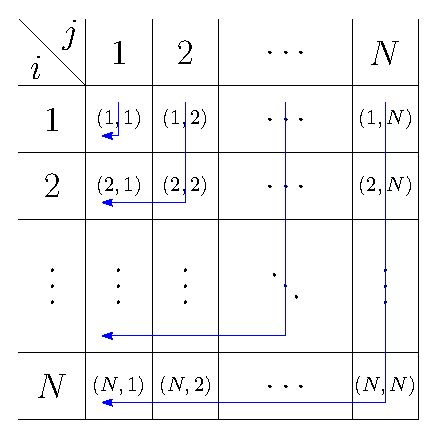
\includegraphics[width=0.3\textwidth]{MA3L5_1.eps}
		\label{5_1}
		\caption{Нумерация $N^2$ элементов.}
		\label{fig:Нумерация}
	\end{figure}
	Тогда, частичная сумма ряда из попарных произведений будет равна:
	$$
		S_{N^2} = \dsum\limits_{i,j \leq N} a_i b_j = 	\left(\dsum\limits_{i = 1 }^{N}a_i \right) {\cdot} \left(\dsum\limits_{j = 1 }^{N} b_j\right) \to A{\cdot}B
	$$
	Поскольку сумма ряда сходится, то существует предел $S_N$, а так как предел подпоследовательности равен пределу последовательности, то $S_N \to A{\cdot}B$.
\end{proof}

Можно ли ослабить требование абсолютной сходимости ряда? Оказывается, что можно.
\begin{theorem}(\textbf{Мертенс})
	Если $\dsum\limits_{n = 1}^{\infty} a_n$ сходится абсолютно и ряд $\dsum\limits_{n = 1}^{\infty} b_n$ сходится, то ряд $\dsum\limits_{n = 1}^{\infty} c_n$, где:
	$$
		c_n = a_1 b_n + a_2 b_{n-1} + \dotsc + a_n b_1
	$$ 
	сходится к произведению рядов $A = \dsum\limits_{n = 1}^{\infty} a_n$ и $B = \dsum\limits_{n = 1}^{\infty} b_n$:
	$$
		\dsum\limits_{n = 1}^{\infty} c_n  = A{\cdot}B = \left(\dsum\limits_{n = 1}^{\infty} a_n\right){\cdot}\left(\dsum\limits_{n = 1}^{\infty} b_n\right)
	$$
\end{theorem}

Рассмотрим с точки зрения нумерации, каким образом получаются $c_n$? На самом деле, это просто движение по неглавным диагоналям множества $\{(a_i, b_j) \mid 1 \leq i,j \leq N\}$: 
\begin{figure}[H]
	\centering
	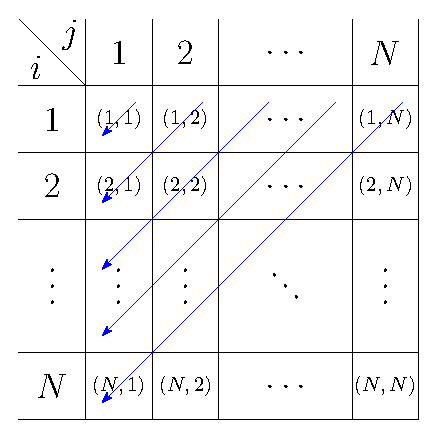
\includegraphics[width=0.3\textwidth]{MA3L5_2.eps}
	\label{5_2}
	\caption{Нумерация элементов $a_i b_j$ в элементе $c_n$.}
	\label{fig:Нумерация}
\end{figure}
Например, $c_1 = a_1 b_1, \, c_2 = a_2 b_1 + a_1 b_2, \, c_3 = a_3 b_1 + a_2 b_2 + a_1 b_3$ и так далее.
\begin{rem}
	Когда нет абсолютной сходимости, это естественно ожидать, что становится важным как складывать слагаемые и надо найти правильный способ как это делать. Почему именно такой способ получился? Возьмем два многочлена и перемножим между собой:
	$$
		(a_1 + a_2x + a_3 x^2 + \dotsc){\cdot}(b_1 + b_2 x + b_3 x^3 + \dotsc)
	$$
	раскроем скобки и приведём подобные:
	$$
		a_1 b_1 + (a_2 b_1 + a_1 b_2) x + (a_3 b_1 + a_2 b_2 + a_1 b_3)x^2  + \dotsc
	$$
	Получается, что мы как-будто взяли ряды $\dsum\limits_{n = 1}^{\infty} a_n x^{n-1}$ и $\dsum\limits_{n = 1}^{\infty} b_n x^{n-1}$, а затем перемножили их как многочлены и привели подобные.
\end{rem}

\begin{proof}
	Рассмотрим частичную сумму ряда $\dsum\limits_{n = 1}^{\infty} c_n$ и подставим в неё значения $c_n$:
	$$
		c_1 + c_2 + \dotsc + c_N = a_1 b_1 + a_2 b_1 + a_1 b_2 + a_3 b_1 + a_2 b_2 + a_1 b_3 + \dotsc + a_N b_1 + \dotsc + a_1 b_N
	$$
	Сгруппируем элементы при $a_i$, тогда получим:
	$$
		c_1 + c_2 + \dotsc + c_N = a_1 (b_1 + b_2 + \dotsc + b_N) + a_2(b_1 + \dotsc + b_{N-1}) + \dotsc + a_n b_1
	$$
	Или, введя обозначение $B_k = b_1 + \dotsc + b_k$, мы получим следующий вид:
	$$
		c_1 + c_2 + \dotsc + c_N = a_1 B_N + a_2 B_{N-1} + \dotsc a_N B_1
	$$
	Мы знаем, что по условию $B_N  \to B$, то есть $B_n = B + \beta_n, \, \lim\limits_{n \to \infty } =0$. Подставим это выражение в частичную сумму рассматриваемого ряда и тогда получим:
	$$
		\sum\limits_{n = 1}^{N} c_n = B{\cdot}(a_1 + \dotsc + a_N) + a_1 \beta_N + a_2 \beta_{N-1} + \dotsc + a_N \beta_1
	$$
	Из условия мы знаем:
	$$
		\lim\limits_{N \to \infty} \dsum\limits_{n = 1}^{N}a_n = A \Rightarrow \lim\limits_{N \to \infty} B{\cdot}(a_1 + \dotsc + a_N) = B{\cdot}A
	$$ 
	Рассмотрим оставшуюся часть частичной суммы: 
	$$
		a_1 \beta_N + a_2 \beta_{N-1} + \dotsc + a_N \beta_1
	$$
	Если мы докажем что она стремится к нулю, то мы получим требуемое. С одной стороны $\beta_n$ - маленькие, поскольку стремтся к нулю, но вплоть до какого-то номера, они маленькими не явлются. Соответствено часть этих слагаемых будет мала за счёт абсолютной сходимости ряда из $a_n$. Оценим эту сумму по частям. Сначала рассмотрим хвостовую часть, затем начальную.
	
	Из абсолютной сходимости имеем $\dsum\limits_{n = 1}^{\infty}|a_n| < \infty$, тогда:
	$$
		\forall \VE > 0, \, \exists \, M \colon \dsum\limits_{n \geq M}|a_n| < \VE
	$$
	Пусть мы нашли этот номер $M$. Поскольку $\beta_n$ стремятся к нулю $\Rightarrow$ они заведомо ограниченны, тогда:
	$$
		\left|a_{M+1} \beta_{M-N} + \dotsc + a_N \beta_1\right| \leq C{\cdot} \sum\limits_{n \geq M}|a_n| < C\VE
	$$
	Зафиксировав номер $M$ и оценива хвостовую часть суммы, мы хотим теперь оценить её начало:
	$$
		\left|a_1 \beta_N + a_2 \beta_{N-1} + \dotsc + a_M \beta_{N - M + 1}\right|
	$$
	Поскольку мы ещё не зафиксировали номер $N$ и последовательность $\beta_n$ стремится к нулю, то возьмем уже зафиксированное $\VE > 0$ и найдем номер $N_0$ такой, что:
	$$
		\exists \, N_0 \colon \forall N > N_0, \, \left|\beta_{N - M + 1}\right| < \dfrac{\VE}{M{\cdot}\max\limits_{k \leq M}\left|a_k\right| + 1}
	$$
	Тогда будет верно:
	$$
		\forall N > N_0, \, |a_1 \beta_N  + \dotsc + a_M \beta_{N - M + 1}| < \dfrac{\VE {\cdot} M{\cdot}\max\limits_{k \leq M}\left|a_k\right|}{M{\cdot}\max\limits_{k \leq M}\left|a_k\right| + 1} < \VE
	$$
	Следовательно, получаем требуемое:
	$$
		\forall N > N_0,\, \left|a_1 \beta_N + \dotsc + a_N \beta_1 \right| < (C + 1)\VE
	$$
\end{proof}

\textbf{Пример}: Рассмотрим произведение следующих рядов (условно сходящихся):
$$
	\dsum\limits_{n = 1}^{\infty}\dfrac{(-1)^n}{\sqrt{n}}{\cdot}\dsum\limits_{n = 1}^{\infty}\dfrac{(-1)^n}{\sqrt{n}} \Rightarrow a_k b_{n - k + 1} =\dfrac{(-1)^k}{\sqrt{k}}{\cdot}\dfrac{(-1)^{n- k + 1}}{\sqrt{n - k +1 }} = \dfrac{(-1)^{n+1}}{\sqrt{k(n - k + 1)}} \Rightarrow
$$
$$
	\Rightarrow c_n = a_1 b_n + \dotsc + a_n b_1 = (-1)^{n+1}{\cdot}\left(\dsum\limits_{k = 1}^n\dfrac{1}{\sqrt{k(n - k + 1)}}\right)
$$
Как понять, сходится ли этот ряд? Для этого нужно рассмотреть $k(n-k + 1) = k((n+1) - k) =f(k)$. Следовательно $f(k)$ вогнутая и достигает максимума в точке $k = \dfrac{n+1}{2}$. Тогда: 
$$
	k(n - k + 1) \leq \dfrac{n+1}{2}\left(\dfrac{n+1}{2}\right) = \dfrac{(n+1)^2}{4} \Rightarrow \dfrac{1}{\sqrt{k(n-k+1)}} \geq \dfrac{2}{n + 1}
$$
Таким образом, мы получаем следующие неравенства из рядов:
$$
	\dsum\limits_{k = 1}^{n} \dfrac{1}{\sqrt{k(n - k + 1)}} \geq \dsum\limits_{k = 1}^{n} \dfrac{2}{n+1} = \dfrac{2n}{n + 1} \geq 1 \Rightarrow \lim\limits_{n \to \infty} c_n  \neq 0
$$
То есть, не выполняется необходимый признак сходимости ряда $\Rightarrow$ ряд расходится. Из этого мы делаем вывод, что просто так перемножать условно сходящиеся ряды нельзя. Но если всё-таки такое перемножение сойдется, то обязательно к произведению. О чём говорит следующая теорема.

\begin{theorem}(\textbf{Абель})
	Если ряд $\dsum\limits_{n = 1}^{\infty} a_n$ сходится, ряд $\dsum\limits_{n = 1}^{\infty} b_n$ сходится и ряд $\dsum\limits_{n = 1}^{\infty} c_n$ сходится, где:
	$$
		c_n = a_1 b_n + a_2 b_{n-1} + \dotsc + a_n b_1
	$$
	то последний ряд сходится к произведению первых рядов $A = \dsum\limits_{n = 1}^{\infty} a_n$ и $B = \dsum\limits_{n = 1}^{\infty} b_n$: 
	$$
		\dsum\limits_{n = 1}^{\infty} c_n  = A{\cdot}B
	$$
\end{theorem}
\begin{proof}
	Аналогично доказательству предыдущей теоремы, возьмем частичную сумму ряда из $c_n$:
	$$
		C_n = c_1 + \dotsc + c_n = a_1 B_n + \dotsc + a_n B_1
	$$
	Просуммируем все частные суммы и разделим на $n$:
	$$
		\dfrac{C_1 + \dotsc + C_n}{n} = \dfrac{a_1 B_1 + a_2 B_1 + a_1 B_2 + \dotsc + a_1 B_n + \dotsc + a_n B_1}{n} = \dfrac{A_1 B_n + A_2 B_{n-1} + \dotsc + A_n B_1}{n}
	$$
	Мы знаем, что ряд из $c_n$ сходится $\Rightarrow C_n$ стремится к некоторому пределу. По теореме Чезаро (доказывается в курсе Солодова за $1$-ый семестр), если последовательность сходится, то арифметическое среднее её членов также сходится к этому пределу:
	$$
		\lim\limits_{n \to \infty}C_n = C \Rightarrow \lim\limits_{n \to \infty}\dfrac{C_1 + \dotsc + C_n}{n} =  \lim\limits_{n \to \infty}\dfrac{A_1 B_n + \dotsc + A_n B_1}{n} = C
	$$
	А поскольку $A_n \to A$ и $B_n \to B$, то нам нужно показать, что:
	$$
		\dfrac{A_1 B_n + \dotsc + A_n B_1}{n} \to A{\cdot}B
	$$
	Рассмотрим следующую разность:
	$$
		\dfrac{A_1 B_n + \dotsc + A_n B_1}{n} - AB = \dfrac{A_1 (B_n - B) + \dotsc + A_n (B_1 - B) + B(A_1 + \dotsc + A_n) -n AB}{n} =
	$$
	$$
		= \dfrac{A_1 (B_n - B) + \dotsc + A_n (B_1 - B)}{n} + B\left(\dfrac{A_1 + \dotsc + A_n}{n} - AB\right)
	$$
	$$
		\lim\limits_{n \to \infty}B\left(\dfrac{A_1 + \dotsc + A_n}{n} - AB\right) = 0
	$$
	Теперь нам необходимо оценить левую дробь выражения выше. Поскольку $(B_n - B)$ стремятся к нулю, то будет верно: 
	$$
		\forall \VE > 0, \, \exists \, N \colon \forall n > N,\, |B_n - B| < \VE
	$$ 
	Зафиксируем $\VE > 0$, найдем нужное $N$ и тогда оценим одну часть рассматриваемой дроби:
	$$
		\left| \dfrac{A_1 (B_n - B) + \dotsc + A_{n-N} (B_{N + 1} - B)}{n}\right| \leq \VE{\cdot}\dfrac{|A_1| + \dotsc + |A_n| }{n} \leq \VE C
	$$
	где последнее верно в силу ограниченности сходящегося среднего арифметического из $A_n$. Зафиксировав $N$ и заметив, что все оставшиеся слагаемые ограничены, будет верно:
	$$
		\left| \dfrac{A_{n - N + 1} (B_{N} - B) + \dotsc + A_{n} (B_{1} - B)}{n}\right| \leq \dfrac{NC}{n} \to 0 \Rightarrow
	$$
	Таким образом получим:
	$$
		\forall \VE > 0, \, \exists \, N \colon \forall n > N,\, \left|\dfrac{A_1 B_n + \dotsc + A_n B_1}{n} - AB \right| < \VE
	$$
\end{proof}
\newpage
\section*{Несобственный интеграл}
Пусть $f$ определена на $[a,b)$ и $\forall c \in [a,b)$ функция $f$ интегрируема по Риману на отрезке $[a,c]$. Определим функцию:
$$
	F(c) = \ddint{a}{c} f(x)dx
$$

\begin{defn}
	Если существует предел $\lim\limits_{c \to b-} F(c)$, то он называется \uwave{несобственным интегралом Римана} по полуинтервалу $[a,b)$ и обозначается следующим образом:
	$$
		\lim\limits_{c \to b-} F(c) = \ddint{a}{b} f(x)dx
	$$
	при этом говорят, что несобственный интеграл \uwave{сходится}.
\end{defn}

\begin{rem}
	Зачем придумывать такую конструкцию? Есть случаи, когда возникают выражения к которым интеграл Римана неприменим, например для неограниченных выражений.
\end{rem}

\textbf{Пример}: Рассмотрим интеграл:
$$
	\ddint{0}{1}\dfrac{dx}{x^p}
$$
Этот интеграл перестает быть интегралом Римана при $p > 0$, поскольку функция под интегралом перестает быть ограниченной на $[0,1]$. Естественный подход - отойти от особенности:
$$
	\ddint{0}{1}\dfrac{dx}{x^p} = \lim\limits_{c \to 0+} \ddint{c}{1} \dfrac{dx}{x^p} = \lim\limits_{c \to 0+}
	\begin{cases}
		p =1, & -\ln{c} \\
		p \neq 1, & \left. \dfrac{x^{-p + 1}}{-p + 1}\right|_c^1 = \dfrac{1}{-p +1} - \dfrac{c^{-p+1}}{-p + 1}
	\end{cases}
	=
	\begin{cases}
		\infty, &p = 1 \\
		\dfrac{1}{-p +1} , & -p + 1 > 0 \\
		\infty, & -p + 1 < 0
	\end{cases}
$$
Значит этот интеграл сходится при $p < 1$.

\begin{rem}
	Есть другая ситуация в которой появляется необходимость в несобственном интеграле: когда промежуток интегрирования стал не отрезком, а, например, лучом. Такая ситуация также не покрывается интегралом Римана.
\end{rem}
\textbf{Пример}: Рассмотрим интеграл:
$$
	\ddint{1}{+\infty}\dfrac{dx}{x^p}
$$
Здесь подход аналогичен предыдущему примеру:
$$
	\ddint{1}{+\infty}\dfrac{dx}{x^p} = \lim\limits_{c \to +\infty} \ddint{1}{c}\dfrac{dx}{x^p} = \lim\limits_{c \to +\infty}
	\begin{cases}
		p = 1, & -\ln{c} \\
		p \neq 1, & \left. \dfrac{x^{-p + 1}}{-p + 1}\right|_1^c =  \dfrac{c^{-p+1}}{-p + 1} - \dfrac{1}{-p +1}
	\end{cases}
	=
	\begin{cases}
		\infty, &p = 1 \\
		\infty, & -p + 1 > 0 \\
		\dfrac{1}{p - 1} , & -p + 1 < 0
	\end{cases}
$$	
Таким образом, интеграл сходится только, если $p > 1$.
\begin{rem}
	В некоторых текстах эти интегралы разделяют на интегралы $1$-го и $2$-го рода. Мы этого делать не будем.
\end{rem}

\begin{prop}
	Если $f$ интегрируема по Риману на $[a,b]$, то $f$ интегрируема по Риману в несобственном смысле на $[a,b)$ и интегралы совпадают:
	$$
		\ddint{a}{b}f(x)dx = \lim\limits_{c \to b-}F(c)
	$$
\end{prop}
\begin{proof}
	Функция $F(c) = \ddint{a}{c}f(x)dx$ - непрерывна на $[a,b]$. Следовательно:
	$$
		\lim\limits_{c \to b-}F(c) = F(b) = \ddint{a}{b}f(x)dx
	$$
\end{proof}
\begin{rem}
	Более того, функция $F(c)$ - Липшецова, см. лекцию $23$ за прошлый семестр.
\end{rem}
Поскольку несобственный интеграл это предел, то всё, что можно достичь предельным переходом, переносится с обычных интегралов на несобственные. Например, линейность.

\textbf{Линейность}: Если $f$ и $g$ интегрируемы в несобственном смысле на $[a,b)$, то $\forall \alpha, \beta \in \MR$, линейная комбинация этих функций $\alpha f + \beta g$ также интегрируема на $[a,b)$. И верно следующее:
$$
	\ddint{a}{b}\left(\alpha f(x) + \beta g(x)\right)dx = \alpha \ddint{a}{b}f(x)dx + \beta\ddint{a}{b}g(x) dx
$$
\begin{proof}
	Пусть $a < c < b$, тогда по свойству интеграла Римана будет верно:
	$$
		\ddint{a}{c}\left(\alpha f(x) + \beta g(x)\right)dx = \alpha \ddint{a}{c}f(x)dx + \beta\ddint{a}{c}g(x) dx
	$$
	Переходя к пределу и воспользовавшись арифметикой предела функции, мы получим требуемое.
\end{proof}

\end{document}